\chapter{Biển Dirac, khối lượng fermion và spinor bốn thành phần}

\section{Fermion chuyển động sang phải và biển Dirac}

Phương trình Dirac là một phương trình cho fermion. Các boson tương đối tính thỏa mãn những phương trình khác, chẳng hạn như phương trình Klein--Gordon hoặc các phương trình Maxwell. Ví dụ đơn giản nhất xét trong một chiều không gian và ban đầu mô tả các hạt và phản hạt chỉ có thể chuyển động sang phải.

Bắt đầu với một sóng phẳng,
\begin{equation}
\psi(x,t)=\psi_0 e^{i(kx-\omega t)}.
\end{equation}
Vận tốc pha của nó là
\begin{equation}
v_{\mathrm{ph}}=\frac{\omega}{k}.
\end{equation}
Dấu của \(k\) và \(\omega\) là quan trọng. Nếu chúng có cùng dấu, pha truyền sang phải; nếu chúng trái dấu, pha truyền sang trái. Khi \(\omega\) tỉ lệ với \(k\), vận tốc pha và vận tốc nhóm trùng nhau:
\begin{equation}
v_{\mathrm{g}}=\frac{d\omega}{dk}=\frac{\omega}{k}.
\end{equation}

Xét phương trình bậc nhất
\begin{equation}
\frac{\partial\psi}{\partial x}
+
\frac{\partial\psi}{\partial t}
=0.
\end{equation}
Thế sóng phẳng vào cho
\begin{equation}
ik\psi-i\omega\psi=0,
\end{equation}
và do đó
\begin{equation}
\omega=k.
\end{equation}
Vì vậy sóng truyền sang phải. Sẽ thuận tiện nếu gán nhãn trường cho phù hợp:
\begin{equation}
\frac{\partial\psi_R}{\partial t}
=
-\frac{\partial\psi_R}{\partial x}.
\end{equation}

Khôi phục tốc độ ánh sáng cho dạng có thứ nguyên
\begin{equation}
\frac{\partial\psi_R}{\partial x}
+
\frac{1}{c}\frac{\partial\psi_R}{\partial t}
=0,
\end{equation}
để rồi
\begin{equation}
\omega=ck.
\end{equation}
Từ đây trở đi \(c=1\). Với \(\hbar=1\), \(\omega\) cũng là năng lượng của một lượng tử.

\begin{figure}[htbp]
\centering
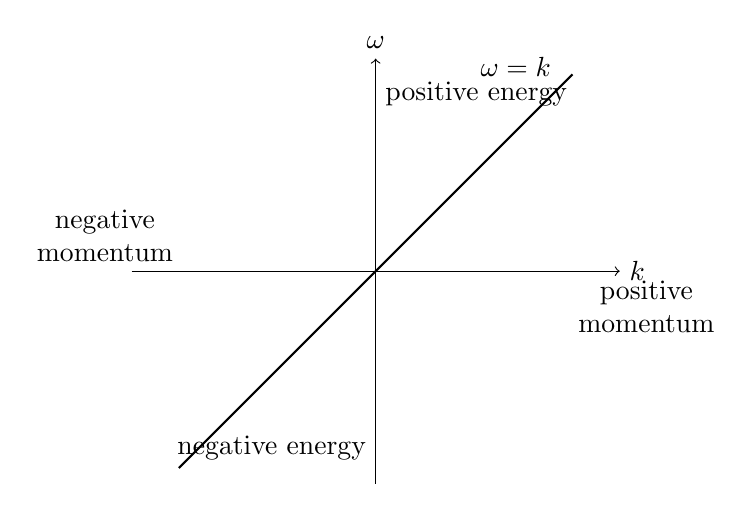
\begin{tikzpicture}[scale=1.0]
\draw[->] (-3.1,0) -- (3.1,0) node[right] {$k$};
\draw[->] (0,-2.7) -- (0,2.7) node[above] {$\omega$};
\draw[thick] (-2.5,-2.5) -- (2.5,2.5);
\node[above left] at (2.35,2.35) {$\omega=k$};
\node[below right,align=center] at (2.45,0) {positive\\momentum};
\node[above left,align=center] at (-2.45,0) {negative\\momentum};
\node[right] at (0,2.25) {positive energy};
\node[left] at (0,-2.25) {negative energy};
\end{tikzpicture}
\caption{Quan hệ tán sắc không khối lượng cho chuyển động sang phải \(\omega=k\) có các nhánh năng lượng dương và âm.}
\end{figure}

Đường thẳng này có một hệ quả nghiêm trọng. \(k\) dương cho năng lượng dương, còn \(k\) âm cho năng lượng âm. Tuy vậy, cả hai phần vẫn mô tả các sóng truyền sang phải vì \(\omega/k=1\) trên toàn bộ đường thẳng.

Một electron đặt trên phần năng lượng dương có thể rơi xuống một trạng thái thấp hơn, phát ra một photon năng lượng dương, lại rơi xuống, rồi tiếp tục đi xuống phổ: xuống một bậc, rồi một bậc nữa, rồi thêm một bậc nữa. Sẽ không electron nào ổn định. Nghiêm trọng hơn, thế giới sẽ hạ năng lượng của mình bằng cách tạo ra ngày càng nhiều electron năng lượng âm.

Nguyên lý loại trừ fermion cung cấp cách chữa. Hãy lấp đầy mọi trạng thái electron năng lượng âm. Không electron thứ hai nào có thể đi vào một trạng thái đã bị chiếm, nên miền năng lượng âm đã lấp đầy hoàn toàn chặn một sự rơi xuống vô hạn. Miền đã lấp đầy này là biển Dirac, và trạng thái lấp đầy hoàn toàn của nó là trạng thái cơ bản, hay chân không.

\begin{classroomqa}
\lecturetimestamp{00:07:19}
\audiencequestion{Có vô hạn nhiều trạng thái năng lượng âm thấp hơn không?}
\lecturerresponse{Có. Với xung lượng rời rạc, phổ giống như một cầu thang vô hạn; với xung lượng liên tục, nó giống như một dốc trượt liên tục. Việc lấp đầy biển năng lượng âm ngăn một electron đi xuống vô hạn định, mặc dù một chuyển mức đi xuống hữu hạn kèm phát xạ photon vẫn có thể xảy ra khi có sẵn một trạng thái thấp hơn chưa bị chiếm.}
\end{classroomqa}

Điều này giải thích vì sao một phương trình có phổ như vậy phải được lượng tử hóa như một lý thuyết fermion. Nếu các lượng tử là boson, thì có thể có tùy ý nhiều lượng tử cùng chiếm một trạng thái thấp hơn ấy, và việc lấp đầy miền năng lượng âm sẽ không làm ổn định chân không.

Bức tranh biển lấp đầy cũng tạo ra phản hạt. Trong chân không, mọi mức năng lượng âm đều bị chiếm và mọi mức năng lượng dương đều trống. Có thể kích một electron từ bất kỳ mức năng lượng âm bị chiếm nào lên bất kỳ mức năng lượng dương chưa bị chiếm nào; các mức ban đầu và cuối không nhất thiết phải nằm đối xứng.

\begin{figure}[htbp]
\centering
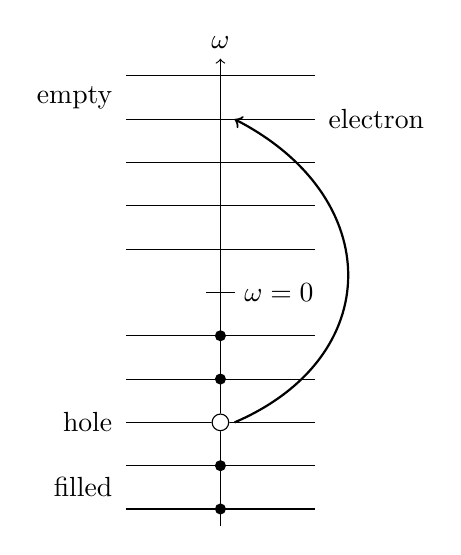
\begin{tikzpicture}[x=1cm,y=0.55cm]
\draw[->] (0,-5.4) -- (0,5.4) node[above] {$\omega$};
\draw (-0.18,0) -- (0.18,0) node[right] {$\omega=0$};
\foreach \y in {-5,-4,-3,-2,-1} {
  \draw (-1.2,\y) -- (1.2,\y);
  \fill (0,\y) circle (2pt);
}
\foreach \y in {1,2,3,4,5} {
  \draw (-1.2,\y) -- (1.2,\y);
}
\draw[->,thick] (0.18,-3) .. controls (2.1,-1.5) and (2.1,2.2) .. (0.18,4);
\draw[white,fill=white] (0,-3) circle (3pt);
\draw (0,-3) circle (3pt);
\node[left] at (-1.25,-3) {hole};
\node[left] at (-1.25,-4.5) {filled};
\node[left] at (-1.25,4.5) {empty};
\node[right] at (1.25,4) {electron};
\end{tikzpicture}
\caption{Kích một electron năng lượng âm đang chiếm tạo ra một electron năng lượng dương và để lại một lỗ trống trong biển đã lấp đầy.}
\end{figure}

Việc lấy đi một electron có năng lượng âm làm tăng năng lượng so với chân không, nên lỗ trống có năng lượng dương. Trên nhánh \(\omega=k\), electron bị lấy đi cũng có xung lượng âm. Việc loại bỏ xung lượng âm để lại một phần dư xung lượng dương, nên lỗ trống có xung lượng dương. Nếu quy ước điện tích electron là âm, electron bị thiếu có điện tích dương. Vì thế lỗ trống là một phản hạt có năng lượng dương và xung lượng dương, còn electron được kích lên có điện tích âm, năng lượng dương và xung lượng dương. Mọi kích thích thực trong lý thuyết một nhánh này đều chuyển động sang phải.

Trường \(\psi_R\) được xây dựng từ các toán tử tạo và hủy fermion. Vì thế cách hiểu hạt và lỗ trống là một phát biểu về các lượng tử mà trường tạo ra và hủy đi, chứ không chỉ về một sóng cổ điển.

Vẫn còn một sự bất đối xứng. Biển chuyển động sang phải chứa các trạng thái năng lượng âm có xung lượng âm. Tổng xung lượng hình thức của nó là rất lớn và hướng sang trái. Có thể định nghĩa xung lượng chân không bằng 0 bằng cách trừ đi hằng số đó, nhưng trạng thái ấy vẫn mất cân bằng về mặt cấu trúc: hạt và phản hạt chỉ chuyển động sang phải, trong khi chân không đã lấp đầy lại được tạo nên từ các trạng thái xung lượng âm.

\section{Nhánh chuyển động sang trái và chân không cân bằng}

Cân bằng trái-phải đòi hỏi một trường thứ hai, độc lập, với các toán tử tạo và hủy riêng của nó. Cho trường đó thỏa mãn
\begin{equation}
\frac{\partial\psi_L}{\partial t}
=
+\frac{\partial\psi_L}{\partial x}.
\end{equation}
Với cùng dạng sóng phẳng,
\begin{equation}
-i\omega\psi_L=ik\psi_L,
\end{equation}
nên
\begin{equation}
\omega=-k.
\end{equation}
Đường thẳng thứ hai này là ảnh gương của \(\omega=k\). Nhánh năng lượng dương của nó mô tả các hạt chuyển động sang trái, và nhánh năng lượng âm của nó cũng phải được lấp đầy.

\begin{figure}[htbp]
\centering
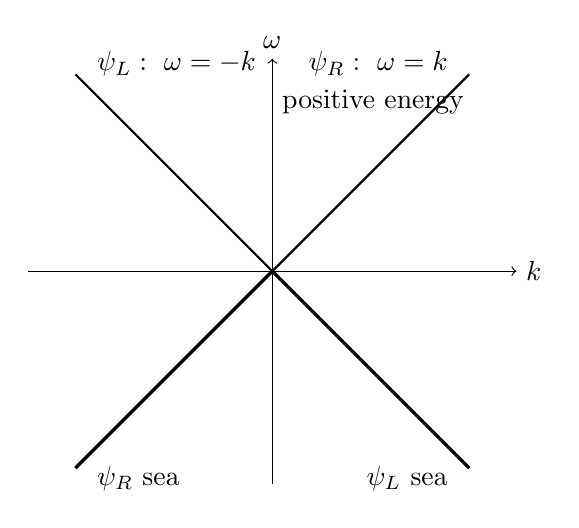
\begin{tikzpicture}[scale=1.0]
\draw[->] (-3.1,0) -- (3.1,0) node[right] {$k$};
\draw[->] (0,-2.7) -- (0,2.7) node[above] {$\omega$};
\draw[thick] (-2.5,-2.5) -- (2.5,2.5);
\draw[thick] (-2.5,2.5) -- (2.5,-2.5);
\draw[very thick] (-2.5,-2.5) -- (0,0);
\draw[very thick] (0,0) -- (2.5,-2.5);
\node[above left] at (2.35,2.35) {$\psi_R:\ \omega=k$};
\node[above right] at (-2.35,2.35) {$\psi_L:\ \omega=-k$};
\node[right] at (0,2.15) {positive energy};
\node[below right] at (-2.35,-2.35) {$\psi_R$ sea};
\node[below left] at (2.35,-2.35) {$\psi_L$ sea};
\end{tikzpicture}
\caption{Các trường độc lập chuyển động sang phải và sang trái cho hai nhánh không khối lượng đối xứng gương; hai bán nhánh năng lượng âm được lấp đầy trong chân không.}
\end{figure}

Sau khi lấp đầy cả hai biển năng lượng âm, số trạng thái bị chiếm chuyển động sang trái bằng số trạng thái bị chiếm chuyển động sang phải. Các xung lượng chân không của chúng cân bằng nhau. Các kích thích hạt và lỗ trống nay có thể chuyển động theo cả hai hướng.

\begin{classroomqa}
\lecturetimestamp{00:15:58}
\audiencequestion{Có thể xử lý bài toán năng lượng âm mà không cần giả định các trạng thái lấp đầy và lỗ trống không?}
\lecturerresponse{Có thể gán nhãn lại cho chính lý thuyết ấy. Một trạng thái electron năng lượng âm đã lấp đầy có thể được gọi là một trạng thái phản hạt trống; khi đó ngôn ngữ vật lý chỉ còn các hạt và phản hạt năng lượng dương. Bức tranh biển lấp đầy vẫn là một phép kiểm tra tính nhất quán hữu ích, khá giống một dải đã lấp đầy trong kim loại, nơi việc lấy đi một electron tạo ra một lỗ trống còn việc kích lên tạo ra cả một hạt lẫn một lỗ trống.}
\end{classroomqa}

Các kích thích đã xét cho đến nay đều không khối lượng. Quan hệ tán sắc của chúng là tuyến tính và vận tốc của chúng có độ lớn \(1\), nên chúng chuyển động với tốc độ ánh sáng. Câu hỏi tiếp theo là làm thế nào để gán khối lượng cho chúng.

\section{Hai thành phần và số hạng khối lượng}

Trước hết gộp hai trường thành một vectơ cột:
\begin{equation}
\Psi=
\begin{pmatrix}
\psi_R\\
\psi_L
\end{pmatrix}.
\end{equation}
Ban đầu đây chỉ là ký hiệu gọn cho hai phương trình độc lập. Định nghĩa
\begin{equation}
\alpha=
\begin{pmatrix}
1&0\\
0&-1
\end{pmatrix}.
\end{equation}
Khi đó các phương trình chuyển động sang phải và sang trái trở thành
\begin{equation}
\frac{\partial\Psi}{\partial t}
=
-\alpha\frac{\partial\Psi}{\partial x}.
\end{equation}

\begin{figure}[htbp]
\centering
\includegraphics[width=0.78\textwidth]{lecture_06_figure_02.png}
\caption{Các trường \(\psi_R\) và \(\psi_L\) tạo thành một spinor hai thành phần, với \(\alpha\) dùng để phân biệt hai nhánh không khối lượng.}
\lectureframe{00:20:36}
\end{figure}

Đối với một sóng phẳng, các toán tử
\begin{equation}
i\partial_t
\quad\hbox{and}\quad
-i\partial_x
\end{equation}
cho ra lần lượt \(\omega\) và \(k\). Vì thế phương trình ma trận có thể được viết gọn thành
\begin{equation}
\omega=\alpha k.
\end{equation}
Đối với thành phần trên, điều này cho \(\omega=k\); đối với thành phần dưới, nó cho \(\omega=-k\). Ký hiệu này đã nén gọn hai phương trình nhưng không đưa thêm vật lý mới nào.

Electron không phải là không khối lượng và không chuyển động với tốc độ ánh sáng. Một công thức dễ khiến ta nghĩ tới cho năng lượng của chúng là động năng phi tương đối tính \(k^2/(2m)\), nhưng ở đây đó không thể là điểm khởi đầu: giới hạn không khối lượng đã liên quan đến chuyển động với tốc độ ánh sáng. Hệ thức tương đối tính là
\begin{equation}
\omega^2=k^2+m^2,
\end{equation}
hoặc, nếu kể cả hai nhánh năng lượng,
\begin{equation}
\omega=\pm\sqrt{k^2+m^2}.
\end{equation}
Khi \(m=0\), các hệ thức này rút về \(\omega=k\) và \(\omega=-k\).

\begin{classroomqa}
\lecturetimestamp{00:25:23}
\audiencequestion{Ở đây có đang dùng đơn vị \(c=1\) không, và tốc độ của một hạt có khối lượng được suy ra như thế nào?}
\lecturerresponse{Có. Tốc độ của một gói sóng là vận tốc nhóm, \(v_{\mathrm g}=d\omega/dk=k/\sqrt{k^2+m^2}\) trên nhánh năng lượng dương. Vì vậy bản thân quan hệ tán sắc đã chứa sự giảm của tốc độ xuống dưới \(c=1\) đối với một hạt có khối lượng.}
\end{classroomqa}

\begin{classroomqa}
\lecturetimestamp{00:26:29}
\audiencequestion{Trong ký hiệu viết gọn \(\omega=\alpha k\), \(\omega\) là một vectơ hay một ma trận?}
\lecturerresponse{Ký hiệu viết gọn đó biểu diễn một phương trình toán tử tác dụng lên hàm sóng hai thành phần. Ở đây \(\omega\) có nghĩa là \(i\partial_t\), \(k\) có nghĩa là \(-i\partial_x\), và \(\alpha\) là ma trận tác dụng lên chỉ số thành phần. Các ký hiệu vô hướng \(\omega\) và \(k\) chỉ trở thành các trị riêng số của chúng trên một sóng phẳng.}
\end{classroomqa}

Giữ phương trình ở bậc nhất và thử phần mở rộng phụ thuộc khối lượng đơn giản nhất:
\begin{equation}
\omega=\alpha k+\beta m.
\end{equation}
Đối tượng \(\beta\) phải là một ma trận vì nó tác dụng lên cùng trường hai thành phần như \(\alpha\). Đại số của nó suy ra bằng cách bình phương:
\begin{align}
\omega^2
&=(\alpha k+\beta m)(\alpha k+\beta m)\\
&=\alpha^2k^2+\beta^2m^2
+\alpha\beta\,km+\beta\alpha\,mk\\
&=\alpha^2k^2+\beta^2m^2
+(\alpha\beta+\beta\alpha)km.
\end{align}
Để thu được \(k^2+m^2\) với mọi \(k\) và \(m\), cần có
\begin{equation}
\alpha^2=I,
\qquad
\beta^2=I,
\qquad
\alpha\beta+\beta\alpha=0.
\end{equation}

Hai số thông thường khác không không thể thỏa mãn điều kiện cuối cùng: đối với các số, điều đó sẽ cho \(2\alpha\beta=0\), trái với việc bình phương của cả hai đều bằng \(1\). Các ma trận có thể phản giao hoán. Cụ thể, \(\beta\) không thể bằng \(\alpha\), vì khi đó
\begin{equation}
\alpha\beta+\beta\alpha=2\alpha^2=2I.
\end{equation}

Chọn
\begin{equation}
\beta=
\begin{pmatrix}
0&1\\
1&0
\end{pmatrix}.
\end{equation}
Bình phương của nó có thể được kiểm tra từng phần tử một:
\begin{equation}
\begin{aligned}
\beta^2
&=
\begin{pmatrix}
0&1\\
1&0
\end{pmatrix}
\begin{pmatrix}
0&1\\
1&0
\end{pmatrix}\\
&=
\begin{pmatrix}
0\cdot0+1\cdot1&0\cdot1+1\cdot0\\
1\cdot0+0\cdot1&1\cdot1+0\cdot0
\end{pmatrix}
=
\begin{pmatrix}
1&0\\
0&1
\end{pmatrix}.
\end{aligned}
\end{equation}
Thứ tự nhân là quan trọng:
\begin{align}
\alpha\beta
&=
\begin{pmatrix}
1&0\\
0&-1
\end{pmatrix}
\begin{pmatrix}
0&1\\
1&0
\end{pmatrix}
=
\begin{pmatrix}
0&1\\
-1&0
\end{pmatrix},\\
\beta\alpha
&=
\begin{pmatrix}
0&1\\
1&0
\end{pmatrix}
\begin{pmatrix}
1&0\\
0&-1
\end{pmatrix}
=
\begin{pmatrix}
0&-1\\
1&0
\end{pmatrix}.
\end{align}
Do đó
\begin{equation}
\alpha\beta=-\beta\alpha,
\qquad
\alpha\beta+\beta\alpha=0.
\end{equation}
Có thể chọn những ma trận tương đương khác, nhưng lựa chọn này làm cho các phương trình thành phần đặc biệt rõ ràng.

Khôi phục các toán tử vi phân cho ta phương trình có khối lượng
\begin{equation}
i\frac{\partial\Psi}{\partial t}
=
-i\alpha\frac{\partial\Psi}{\partial x}
+m\beta\Psi.
\end{equation}
Ma trận \(\beta\) hoán đổi hai thành phần:
\begin{equation}
\beta
\begin{pmatrix}
\psi_R\\
\psi_L
\end{pmatrix}
=
\begin{pmatrix}
\psi_L\\
\psi_R
\end{pmatrix}.
\end{equation}
Do đó,
\begin{align}
i\dot{\psi}_R
&=-i\frac{\partial\psi_R}{\partial x}+m\psi_L,\\
i\dot{\psi}_L
&=+i\frac{\partial\psi_L}{\partial x}+m\psi_R.
\end{align}

Số hạng khối lượng ghép cặp các trường vốn độc lập trong lý thuyết không khối lượng. Phương trình cho thành phần trên chứa thành phần dưới, và phương trình cho thành phần dưới chứa thành phần trên. Sự ghép cặp này chính là ý nghĩa của khối lượng Dirac. Các phương trình là bất biến theo tịnh tiến, nên chúng bảo toàn xung lượng, và khối lượng của các kích thích hạt của chúng là \(m\).

\begin{classroomqa}
\lecturetimestamp{00:38:25}
\audiencequestion{Một nghiệm có tự động bất biến Lorentz không?}
\lecturerresponse{Một nghiệm cụ thể không nên giữ nguyên dưới một phép biến đổi Lorentz. Một trạng thái có một xung lượng được biến đổi thành một trạng thái có xung lượng đã biến đổi, nên phát biểu thích hợp là tính hiệp biến. Hệ thức \(\omega^2=k^2+m^2\) là một phép kiểm tra bất biến Lorentz then chốt, nhưng hiệp biến đầy đủ còn đòi hỏi quy luật biến đổi của spinor \(\Psi\), điều mà đến nay vẫn chưa được thiết lập.}
\end{classroomqa}

\section{Hệ quy chiếu nghỉ và ý nghĩa của các thành phần}

Không thể đưa một hạt không khối lượng về đứng yên, nhưng có thể làm vậy với một hạt có khối lượng. Ở trạng thái nghỉ \(k=0\), nên hàm sóng không có biến thiên theo không gian và
\begin{equation}
\omega=\beta m.
\end{equation}
Phương trình vi phân rút gọn thành
\begin{equation}
i\frac{d\Psi}{dt}=m\beta\Psi.
\end{equation}
Viết theo các thành phần,
\begin{align}
i\dot{\psi}_R&=m\psi_L,\\
i\dot{\psi}_L&=m\psi_R.
\end{align}
Cả hai phần tử ngoài đường chéo của \(\beta\) đều là \(+1\), nên trong cả hai phương trình này đều không có thêm dấu trừ.

Các phương trình tách rời sau khi cộng và trừ các thành phần. Định nghĩa
\begin{equation}
\psi_+=\psi_R+\psi_L,
\qquad
\psi_-=\psi_R-\psi_L.
\end{equation}
Cộng hai phương trình trong hệ quy chiếu nghỉ cho
\begin{equation}
i\dot{\psi}_+=m\psi_+,
\end{equation}
trong khi lấy hiệu của chúng cho
\begin{equation}
i\dot{\psi}_-=-m\psi_-.
\end{equation}
Vì thế
\begin{equation}
\omega=+m
\quad\hbox{for }\psi_+,
\qquad
\omega=-m
\quad\hbox{for }\psi_-.
\end{equation}

\begin{figure}[htbp]
\centering
\includegraphics[width=0.62\textwidth]{lecture_06_figure_03.png}
\caption{Ở xung lượng bằng 0, \(\psi_+=\psi_R+\psi_L\) và \(\psi_-=\psi_R-\psi_L\) có các tần số nghỉ \(\omega=+m\) và \(\omega=-m\).}
\lectureframe{00:44:49}
\end{figure}

Trường ở trạng thái nghỉ có năng lượng dương là \(\psi_+\); trường ở trạng thái nghỉ có năng lượng âm là \(\psi_-\). Các trạng thái năng lượng âm được lấp đầy, đúng như trước. Kết quả trong hệ quy chiếu nghỉ chỉ là lát cắt \(k=0\) của toàn bộ phổ:
\begin{equation}
\omega_\pm(k)=\pm\sqrt{k^2+m^2}.
\end{equation}
\begin{figure}[htbp]
\centering
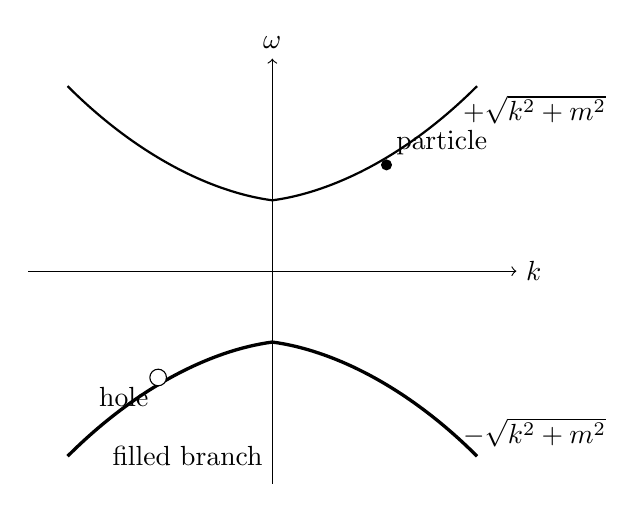
\begin{tikzpicture}[scale=1.0]
\draw[->] (-3.1,0) -- (3.1,0) node[right] {$k$};
\draw[->] (0,-2.7) -- (0,2.7) node[above] {$\omega$};
\draw[thick] (-2.6,2.35)
  .. controls (-1.7,1.45) and (-0.75,1.0) .. (0,0.9)
  .. controls (0.75,1.0) and (1.7,1.45) .. (2.6,2.35);
\draw[very thick] (-2.6,-2.35)
  .. controls (-1.7,-1.45) and (-0.75,-1.0) .. (0,-0.9)
  .. controls (0.75,-1.0) and (1.7,-1.45) .. (2.6,-2.35);
\fill (1.45,1.35) circle (2pt);
\node[above right] at (1.45,1.35) {particle};
\fill[white] (-1.45,-1.35) circle (3pt);
\draw (-1.45,-1.35) circle (3pt);
\node[below left] at (-1.45,-1.35) {hole};
\node[right] at (2.3,2.05) {$+\sqrt{k^2+m^2}$};
\node[right] at (2.3,-2.05) {$-\sqrt{k^2+m^2}$};
\node[left] at (0,-2.35) {filled branch};
\end{tikzpicture}
\caption{Ở mọi xung lượng, phổ có khối lượng đều có các trạng thái năng lượng dương và âm. Nhánh âm được lấp đầy, và một trạng thái bị thiếu trong đó là một lỗ trống năng lượng dương.}
\end{figure}
Mỗi xung lượng đều có một trạng thái năng lượng dương và một trạng thái năng lượng âm. Việc lấp đầy mọi trạng thái trên nhánh âm để lại các hạt năng lượng dương ở phía trên biển và các lỗ trống năng lượng dương ở trong đó. Hạt và lỗ trống đều có khối lượng dương.

Điểm cốt yếu đáng được nhắc lại. Một fermion trở nên có khối lượng khi hai thành phần trước đây độc lập của nó bị ghép cặp. Ở trạng thái nghỉ, không thành phần ban đầu nào riêng lẻ là một trạng thái riêng năng lượng. Các trạng thái năng lượng xác định là tổng và hiệu của chúng.

Để thấy tổng đó có nghĩa gì, hãy dùng \(C_R^\dagger\) và \(C_L^\dagger\) cho các thành phần tạo một hạt tương ứng. Khi tác dụng lên chân không,
\begin{equation}
(C_R^\dagger+C_L^\dagger)\lvert0\rangle
\end{equation}
tạo ra một hạt trong trạng thái chồng chập kết hợp của hai thành phần. Nó không tạo ra hai hạt. Một tích,
\begin{equation}
C_R^\dagger C_L^\dagger\lvert0\rangle,
\end{equation}
chứa hai toán tử tạo và tạo ra một trạng thái hai hạt khi cả hai mode đều khả dụng. Sau khi chuẩn hóa, trạng thái nghỉ có xác suất bằng nhau trong hai thành phần, nhưng toàn bộ sóng ghép xét như một tổng thể lại có động lượng bằng không.

Các nhãn \(R\) và \(L\) chỉ là các nhãn chuyển động theo nghĩa đen khi \(m=0\). Một khi hạng khối lượng xuất hiện, một nghiệm có khối lượng đang chuyển động nhìn chung chứa cả hai thành phần, còn nghiệm nghỉ chứa chúng với độ lớn bằng nhau. Vì vậy, ở đây tốt hơn nên xem \(R\) và \(L\) là các nhãn cho các thành phần spinor trên và dưới.

\begin{figure}[htbp]
\centering
\includegraphics[width=0.78\textwidth]{lecture_06_figure_04.png}
\caption{Với khối lượng khác không, hai thành phần spinor bị ghép với nhau; cách diễn giải chúng là chuyển động sang phải và sang trái chỉ áp dụng trực tiếp trong giới hạn không khối lượng.}
\lectureframe{00:50:48}
\end{figure}

Mọi fermion có khối lượng trong vật lý hạt đều được xây dựng từ các trường thành phần trái và phải: khối lượng Dirac ghép các thành phần vốn độc lập trong giới hạn không khối lượng.

\begin{classroomqa}
\lecturetimestamp{00:52:01}
\audiencequestion{Liệu \(\psi_R\pm\psi_L\) có nên chứa một thừa số \(1/\sqrt{2}\) không?}
\lecturerresponse{Có thể đưa vào để chuẩn hóa trạng thái. Nó nhân vào cả hai vế của phương trình và vì thế không làm thay đổi phương trình chuyển động.}
\end{classroomqa}

\begin{classroomqa}
\lecturetimestamp{00:52:12}
\audiencequestion{Độ lớn tương đối của các thành phần phải và trái có quan trọng không?}
\lecturerresponse{Đối với các trạng thái riêng trong hệ quy chiếu nghỉ đã chọn, độ lớn của chúng bằng nhau. Một chuẩn hóa tổng thể là tùy ý, nhưng độ lớn tương đối được cố định bởi vectơ riêng của \(\beta\).}
\end{classroomqa}

\begin{classroomqa}
\lecturetimestamp{00:52:52}
\audiencequestion{Hai thành phần có thể có một pha tương đối không?}
\lecturerresponse{Có. Các hệ số thực trong \(\psi_R\pm\psi_L\) là hệ quả của việc chọn một \(\beta\) thực. Những ma trận khác có bình phương thành đơn vị và phản giao hoán với \(\alpha\) cũng là những lựa chọn tương đương, và khi đó pha có thể xuất hiện giữa hai thành phần. Một khi đã chọn một biểu diễn, phải dùng nó một cách nhất quán.}
\end{classroomqa}

\begin{classroomqa}
\lecturetimestamp{00:53:43}
\audiencequestion{Sau khi thêm khối lượng, các nhãn ``chuyển động sang trái'' và ``chuyển động sang phải'' có gây hiểu lầm không?}
\lecturerresponse{Có phần như vậy. Chúng mô tả các sóng thực sự chuyển động sang trái và sang phải trong lý thuyết không khối lượng. Với khối lượng khác không, ngay cả một hạt chuyển động theo một hướng nhìn chung cũng chứa cả hai thành phần, nên ``thành phần trên'' và ``thành phần dưới'' là những nhãn an toàn hơn.}
\end{classroomqa}

\begin{classroomqa}
\lecturetimestamp{00:55:01}
\audiencequestion{Một fermion đứng yên đã đòi hỏi mômen động lượng spin chưa?}
\lecturerresponse{Chưa trong mô hình một chiều này. Mômen động lượng không được định nghĩa trong một chiều không gian, nên spin vẫn chưa đi vào phép xây dựng này.}
\end{classroomqa}

\begin{classroomqa}
\lecturetimestamp{00:55:24}
\audiencequestion{Hàm sóng có chứa các toán tử tạo và hủy fermion không?}
\lecturerresponse{Có.}
\end{classroomqa}

\begin{classroomqa}
\lecturetimestamp{00:55:30}
\audiencequestion{Ngoài việc chọn các toán tử tạo và hủy, tính chất fermion đi vào ở đâu?}
\lecturerresponse{Nó đi vào qua các quy tắc tạo--hủy của fermion. Một phương trình có phổ năng lượng âm như thế này phải được lượng tử hóa với các quy tắc đó; các quy tắc chiếm chỗ của boson sẽ khiến chân không mất ổn định. Các boson tương đối tính phải được mô tả bằng một phương trình sóng khác.}
\end{classroomqa}

\begin{classroomqa}
\lecturetimestamp{00:56:20}
\audiencequestion{Một nghiệm có động lượng khác không có thể được biến đổi Lorentz thành nghiệm trong hệ nghỉ không?}
\lecturerresponse{Có. Một phép boost có thể đưa một nghiệm có khối lượng về hệ nghỉ của nó, nhưng để thực hiện phép biến đổi thì cần biết các phép biến đổi Lorentz tác dụng lên spinor \(\Psi\) như thế nào.}
\end{classroomqa}

\section{Khối lượng từ trường chân không vô hướng}

\begin{classroomqa}
\lecturetimestamp{00:58:11}
\audiencequestion{Tương tác với trường Higgs tạo ra hạng khối lượng Dirac như thế nào?}
\lecturerresponse{Hãy thay hệ số khối lượng hằng bằng một sự ghép với một trường vô hướng. Nếu trường đó triệt tiêu trong chân không, fermion vẫn không có khối lượng; nếu nó có một giá trị chân không hằng khác không, thì sự ghép ấy tác dụng đúng như một khối lượng.}
\end{classroomqa}

Gọi \(\phi(x,t)\) là một trường vô hướng có phương trình chuyển động riêng. Trong phương trình Dirac, hãy thay hằng số \(m\) trong hạng khối lượng bằng \(g\phi(x,t)\):\footnote{Hạng tương tác được hiển thị thu được bằng cách thực hiện phép thay thế này trong hạng khối lượng đã được thiết lập trước đó \(m\beta\Psi\).}
\begin{equation}
i\frac{\partial\Psi}{\partial t}
=
-i\alpha\frac{\partial\Psi}{\partial x}
+g\phi(x,t)\,\beta\Psi.
\end{equation}
Khi đó hai phương trình trường được ghép với nhau. Fermion tác dụng lên trường vô hướng, và trường vô hướng tác dụng ngược trở lại lên fermion; xét như một toàn hệ, hệ là phi tuyến mặc dù phương trình Dirac là tuyến tính theo \(\Psi\) đối với \(\phi\) cho trước.

Giả sử trước hết rằng không gian trống có
\begin{equation}
\phi(x,t)=0.
\end{equation}
Khi đó hạng trộn triệt tiêu, các thành phần trên và dưới tách rời nhau, và fermion không có khối lượng. Thay vào đó, hãy giả sử rằng trạng thái năng lượng thấp nhất có một trường vô hướng hằng khác không,
\begin{equation}
\phi(x,t)=\phi_0\neq0.
\end{equation}
Phương trình Dirac trong chân không đó trở thành
\begin{equation}
i\frac{\partial\Psi}{\partial t}
=
-i\alpha\frac{\partial\Psi}{\partial x}
+g\phi_0\,\beta\Psi,
\end{equation}
để rồi
\begin{equation}
m_{\mathrm{eff}}=g\phi_0.
\end{equation}
Vì vậy, một sự ghép giữa một trường boson và một trường fermion, cùng với một giá trị khác không của trường boson trong không gian trống, sinh ra đúng cùng kiểu trộn trái-phải mà trước đây xuất hiện như một khối lượng được viết trực tiếp vào phương trình.

\begin{classroomqa}
\lecturetimestamp{01:01:27}
\audiencequestion{LHC có thể cung cấp bằng chứng cho một trường Higgs khác không trong chân không không?}
\lecturerresponse{Hoàn toàn có thể. Đó là một trong những vấn đề lớn.}
\end{classroomqa}

\begin{classroomqa}
\lecturetimestamp{01:01:32}
\audiencequestion{Có thể nói thêm về cách cơ chế Higgs hoạt động không?}
\lecturerresponse{Một trường vô hướng có năng lượng gắn với sự biến thiên của nó theo không gian và thời gian, và nó cũng có thể có một thế năng cục bộ \(V(\phi)\). Nếu các cực tiểu của thế đó xuất hiện tại các giá trị khác không của \(\phi\), thì chân không chứa một trường khác không. Những dao động đã lượng tử hóa quanh cực tiểu được chọn là các hạt Higgs.}
\end{classroomqa}

Một trường có thể mang năng lượng theo hai cách khác nhau. Một phần năng lượng phụ thuộc vào việc trường biến thiên như thế nào theo không gian và thời gian. Trường Maxwell là ví dụ đối chiếu quen thuộc:
\begin{equation}
\mathcal{E}_{\mathrm{Maxwell}}\propto \mathbf E^2+\mathbf B^2,
\end{equation}
và cả \(\mathbf E\) lẫn \(\mathbf B\) đều được xây dựng từ các đạo hàm của thế điện từ. Vì vậy, phần năng lượng này gắn với sự biến thiên theo không gian và thời gian của trường cơ sở.

Một trường vô hướng cũng có thể có một mật độ thế năng cục bộ,
\begin{equation}
V(\phi),
\end{equation}
phụ thuộc vào chính giá trị của \(\phi\) chứ không phải vào các đạo hàm của nó. Một cách sơ đồ,
\begin{equation}
\mathcal{E}_\phi
=
\mathcal E_{\text{space and time gradients}}+V(\phi).
\end{equation}
Nếu không có một nguyên lý sâu hơn cố định nó, \(V(\phi)\) có thể là bất kỳ hàm hợp lý nào tương thích với các đối xứng của mô hình.

Đối với minh họa đơn giản bằng trường vô hướng thực đang được dùng ở đây, hãy lấy lý thuyết là đối xứng dưới phép
\begin{equation}
\phi\longrightarrow-\phi.
\end{equation}
Khi đó thế phải là hàm chẵn:
\begin{equation}
V(\phi)=V(-\phi).
\end{equation}
Bản thân đối xứng này không cho biết cực tiểu nằm ở đâu. Một khả năng là chỉ có một cực tiểu tại \(\phi=0\). Khả năng khác là một cặp cực tiểu đối xứng tại các giá trị khác không, một dương và một âm.

\begin{figure}[htbp]
\centering
\includegraphics[width=0.72\textwidth]{lecture_06_figure_05.png}
\caption{Cực tiểu tại \(\phi=0\) cho một trường chân không triệt tiêu, còn các cực tiểu đối xứng khác không cho phép một giá trị chân không \(\phi_0\neq0\) và do đó một khối lượng fermion \(g\phi_0\).}
\lectureframe{01:04:47}
\end{figure}

Hai khả năng đó có thể được vẽ mà không cần chốt một dạng đa thức cụ thể cho thế.\footnote{Các đường cong bên dưới chỉ giữ lại đặc điểm định tính của cực tiểu ở tâm và của các cực tiểu liên hệ với nhau bởi đối xứng được dùng trong lập luận.}
\begin{figure}[htbp]
\centering
\resizebox{\linewidth}{!}{%
\begin{tikzpicture}[x=1.35cm,y=1.05cm]
\begin{scope}[shift={(-3.1,0)}]
\draw[->] (-1.7,0) -- (1.7,0) node[right] {$\phi$};
\draw[->] (0,-0.15) -- (0,2.45) node[above] {$V(\phi)$};
\draw[thick] (-1.5,2.05) .. controls (-0.9,0.65) and (-0.45,0.25) .. (0,0.25)
             .. controls (0.45,0.25) and (0.9,0.65) .. (1.5,2.05);
\fill (0,0.25) circle (1.2pt);
\node[below] at (0,0) {$0$};
\end{scope}
\begin{scope}[shift={(3.1,0)}]
\draw[->] (-1.7,0) -- (1.7,0) node[right] {$\phi$};
\draw[->] (0,-0.15) -- (0,2.45) node[above] {$V(\phi)$};
\draw[thick] (-1.55,2.05)
  .. controls (-1.25,0.75) and (-1.0,0.25) .. (-0.75,0.25)
  .. controls (-0.35,0.25) and (-0.25,1.3) .. (0,1.3)
  .. controls (0.25,1.3) and (0.35,0.25) .. (0.75,0.25)
  .. controls (1.0,0.25) and (1.25,0.75) .. (1.55,2.05);
\fill (-0.75,0.25) circle (1.2pt);
\fill (0.75,0.25) circle (1.2pt);
\node[below] at (0,0) {$0$};
\node[below] at (-0.75,0) {$-\phi_0$};
\node[below] at (0.75,0) {$\phi_0$};
\end{scope}
\end{tikzpicture}%
}
\caption{Các thế chẵn có thể có một cực tiểu ở tâm hoặc hai cực tiểu khác không liên hệ với nhau bởi đối xứng.}
\end{figure}

Nếu cực tiểu nằm tại gốc tọa độ, chân không có \(\phi_0=0\), và sự ghép này không cho electron khối lượng. Nếu các cực tiểu ở \(\phi=\pm\phi_0\), chân không sẽ ổn định vào một trong hai giá trị đó. Hai lựa chọn liên hệ với nhau bởi đối xứng, và lựa chọn nào cũng tạo ra một hệ số khác không \(g\phi_0\) trong phương trình Dirac. Vì sao thế có dạng định tính này là một câu hỏi sâu hơn, không được bản thân cơ chế giải quyết.

Trường không nhất thiết phải luôn ở đúng cực tiểu của nó. Nó có thể dao động quanh giá trị đã chọn cũng như một hạt có thể dao động gần đáy của một giếng thế. Lượng tử hóa các dao động ấy cho ra các lượng tử Higgs. Tần số đặc trưng của chúng liên hệ với khối lượng của hạt Higgs: khối lượng lớn có nghĩa là cần một lượng năng lượng lớn để kích thích dù chỉ một lượng tử. Trong chân không, trường đơn giản là nằm gần cực tiểu của nó và cung cấp khối lượng cho fermion. Khi trường rung động, dao động đó là một hạt Higgs.

Sự ghép kéo theo tác dụng và phản tác dụng. Các fermion đáp ứng với giá trị của \(\phi\), nhưng các va chạm fermion đủ năng lượng cũng có thể kích thích trường vô hướng. Một va chạm phải cung cấp năng lượng kích thích; một khi trường dao động, các lượng tử của nó là các hạt Higgs. Cùng trường đó không chỉ ghép với electron mà còn với các trường quark và các trường khác mà nó cung cấp khối lượng.

\begin{classroomqa}
\lecturetimestamp{01:08:14}
\audiencequestion{Nếu trường Higgs rung động hoặc bị dịch chuyển, khối lượng của electron có thay đổi không?}
\lecturerresponse{Có. Vì khối lượng hiệu dụng tỉ lệ với giá trị cục bộ của trường, nên dịch chuyển trường về phía không sẽ làm giảm khối lượng. Giữ một vùng vĩ mô ở xa giá trị chân không sẽ đòi hỏi năng lượng khổng lồ; một vùng đủ lớn cho thí nghiệm như vậy có thể sụp đổ thành một lỗ đen.}
\end{classroomqa}

Thí nghiệm tư duy này rất trực tiếp. Nếu một vùng có thể được giữ gần \(\phi=0\), thì trong vùng đó
\begin{equation}
m_{\mathrm{eff}}=g\phi
\end{equation}
sẽ trở nên nhỏ hoặc triệt tiêu. Một mode Higgs bị kích thích dao động quanh giá trị chân không, còn việc tạo ra và duy trì một độ lệch đáng kể trong toàn bộ một vùng vĩ mô thì đòi hỏi năng lượng khổng lồ. Cái giá thế năng tăng theo thể tích. Từ rất lâu trước khi một vùng như vậy trở thành một phòng thí nghiệm thực tế, năng lượng của nó đã có thể đủ lớn để gây sụp đổ hấp dẫn. Sự thay đổi khối lượng là có thật về nguyên tắc, nhưng việc sắp đặt một thay đổi lớn có thể quan sát được là cực kỳ khó.

\begin{classroomqa}
\lecturetimestamp{01:09:27}
\audiencequestion{Vì sao cần một trường Higgs?}
\lecturerresponse{Vì electron có khối lượng.}
\end{classroomqa}

\begin{classroomqa}
\lecturetimestamp{01:09:41}
\audiencequestion{Mỗi loại hạt có trường Higgs riêng của nó không?}
\lecturerresponse{Không. Trong Mô hình Chuẩn, một trường Higgs cung cấp khối lượng cho electron, quark và các hạt khác tham gia cơ chế này. Các phiên bản siêu đối xứng đòi hỏi hai trường Higgs chứ không phải một trường riêng biệt cho từng loài hạt.}
\end{classroomqa}

Bức tranh một trường chỉ mang tính sơ đồ: trường Higgs đầy đủ có nhiều cấu trúc hơn một số thực đơn \(\phi\). Tuy vậy, điểm cốt yếu vẫn còn nguyên. Một trường chân không chung có thể ghép với các fermion khác nhau với cường độ khác nhau, nên các khối lượng khác nhau không đòi hỏi những trường Higgs khác nhau cho từng loài. Hạt Higgs là một dao động của chính trường đó quanh giá trị chân không của nó.

Vì sao không đơn giản đưa khối lượng electron vào phương trình bằng tay và bỏ hẳn trường Higgs? Câu trả lời liên quan đến các tương tác yếu và sự thống nhất, và sẽ được để lại cho sau.

\begin{classroomqa}
\lecturetimestamp{01:11:16}
\audiencequestion{Trong một lý thuyết siêu đối xứng, có hai sector Higgs không?}
\lecturerresponse{Có. Trong cách phân chia đơn giản dùng ở đây, một sector cung cấp khối lượng cho quark kiểu up và sector kia cho quark kiểu down và electron. Sự nhân đôi này là một đòi hỏi kỹ thuật của siêu đối xứng, chứ không phải một trường Higgs riêng cho từng hạt.}
\end{classroomqa}

\begin{classroomqa}
\lecturetimestamp{01:12:01}
\audiencequestion{Nếu hạt Higgs có khối lượng, thì khối lượng đó đến từ đâu?}
\lecturerresponse{Câu hỏi đó không được giải quyết ở đây. Vấn đề hóc búa hơn là vì sao khối lượng Higgs lại nhỏ đến vậy.}
\end{classroomqa}

Đối xứng gắn liền không thể tách rời với vấn đề khối lượng. Trong mô hình Dirac đơn giản, một đối xứng ngăn các miền trái và phải trộn lẫn với nhau sẽ buộc hệ số của hạng trộn phải triệt tiêu. Nếu chân không tôn trọng đối xứng đó, fermion sẽ không có khối lượng. Giá trị chân không khác không của Higgs phá vỡ đối xứng chân không liên quan và cho phép sự ghép trái-phải:
\begin{equation}
m_{\mathrm{eff}}=g\phi_0\neq0.
\end{equation}
Phép biến đổi đối xứng chính xác không được triển khai ở đây; điểm cốt yếu là hệ quả của nó đối với hạng khối lượng. Các phương trình có thể có đối xứng ấy mặc dù trạng thái năng lượng thấp nhất cụ thể thì không. Chính sự bất đối xứng của chân không này cung cấp khối lượng.

Trong bức tranh điện yếu đang được phác họa, electron và quark nhận được khối lượng theo cách này, cũng như các boson \(W\) và \(Z\). Photon vẫn không có khối lượng. Bản thân hạt Higgs lại là một ngoại lệ khác: nó có thể có khối lượng ngay cả khi không có cùng độ lệch chân không đó, và khối lượng của nó liên quan đến dao động của chính trường của nó chứ không phải sự trộn trái-phải của fermion. Vì vậy, trong cách mô tả này, giá trị chân không của Higgs sinh ra khối lượng của các hạt khác, còn khối lượng của kích thích Higgs lại đặt ra một câu hỏi riêng.

\begin{classroomqa}
\lecturetimestamp{01:15:26}
\audiencequestion{Graviton có khối lượng không?}
\lecturerresponse{Không. Graviton không có khối lượng, giống như photon. Trước đây người ta cũng từng cho rằng neutrino không có khối lượng, nhưng chúng có khối lượng rất nhỏ; theo ngôn ngữ hiện tại, điều đó có nghĩa là các thành phần trái và phải của chúng chỉ có một sự ghép rất nhỏ.}
\end{classroomqa}

Photon và, trong lý thuyết, graviton đều không có khối lượng và chuyển động với tốc độ ánh sáng. Các neutrino không hẳn thuộc loại đó. Khối lượng rất nhỏ của chúng có nghĩa là, trong ngôn ngữ Dirac này, sự ghép nối các thành phần trái và phải của chúng là rất nhỏ. Vì sao nó nhỏ đến vậy lại là một câu hỏi khác.

\section{Phương trình Dirac trong ba chiều không gian}

Trong ba chiều không gian, số sóng trở thành một vectơ sóng,
\begin{equation}
\mathbf{k}=(k_1,k_2,k_3),
\end{equation}
với các thành phần theo các hướng \(x\), \(y\) và \(z\). Quan hệ một chiều có dạng
\begin{equation}
\omega=\alpha k+\beta m,
\end{equation}
và tổng quát hóa tuyến tính đơn giản nhất của nó là
\begin{equation}
\omega
=
\alpha_1 k_1+\alpha_2 k_2+\alpha_3 k_3+\beta m.
\end{equation}
Ở đây \(\alpha_i\) và \(\beta\) là các ma trận. Chúng phải được chọn sao cho
\begin{equation}
\omega^2=k_1^2+k_2^2+k_3^2+m^2.
\end{equation}
Quan hệ tán sắc bất biến này là một điều kiện thiết yếu, mặc dù tự nó chưa phải toàn bộ nội dung của thuyết tương đối.

Bình phương biểu thức tuyến tính cho
\begin{align}
\omega^2
={}&
\alpha_1^2k_1^2+\alpha_2^2k_2^2+\alpha_3^2k_3^2+\beta^2m^2
\nonumber\\
&+(\alpha_1\alpha_2+\alpha_2\alpha_1)k_1k_2
+(\alpha_1\alpha_3+\alpha_3\alpha_1)k_1k_3
\nonumber\\
&+(\alpha_2\alpha_3+\alpha_3\alpha_2)k_2k_3
+\sum_{i=1}^{3}(\alpha_i\beta+\beta\alpha_i)k_i m.
\end{align}
Các hệ số của bình phương các xung lượng và của khối lượng đòi hỏi
\begin{equation}
\alpha_1^2=\alpha_2^2=\alpha_3^2=I,
\qquad
\beta^2=I.
\end{equation}
Các hạng \(k_i k_j\) không mong muốn biến mất nếu các ma trận \(\alpha\) khác nhau phản giao hoán:
\begin{equation}
\alpha_i\alpha_j+\alpha_j\alpha_i=0,
\qquad i\neq j.
\end{equation}
Các hạng hỗn hợp \(k_i m\) biến mất nếu
\begin{equation}
\alpha_i\beta+\beta\alpha_i=0
\qquad
\text{for each }i.
\end{equation}
Vì vậy cả bốn ma trận đều có bình phương bằng ma trận đơn vị, và mọi cặp ma trận phân biệt đều phản giao hoán.

Quả thực tồn tại ba ma trận \(2\times2\) có các tính chất phản giao hoán lẫn nhau như yêu cầu: đó là ba ma trận Pauli. Không có ma trận \(2\times2\) thứ tư nào vừa có bình phương bằng ma trận đơn vị vừa phản giao hoán với cả ba ma trận ấy. Không có biểu diễn \(3\times3\) nào dùng được cả. Biểu diễn khả dĩ đầu tiên dùng các ma trận \(4\times4\), tức các ma trận Dirac.

Việc chuyển từ hai thành phần sang bốn thành phần đặt ra một câu hỏi vật lý. Trong một chiều không gian, hai thành phần ban đầu là các trường chuyển động sang phải và sang trái. Bốn thành phần có nghĩa là gì? Yếu tố mới sẽ là spin, nhưng spin đòi hỏi mômen góc và vì thế cần một thảo luận đúng nghĩa trong ba chiều.

Các ma trận này không duy nhất. Các cách chọn khác nhau là tương đương, gần như theo đúng cách mà những hệ trục tọa độ trực chuẩn khác nhau là tương đương: các phần tử thay đổi, nhưng có một phép biến đổi liên hệ các mô tả và vật lý thì không đổi. Một biểu diễn thuận tiện là\footnote{Các ma trận viết theo từng phần tử ở dưới là khai triển của dạng khối và các ma trận Pauli được hiển thị ngay sau đó; các quan hệ khối ấy được phát biểu tường minh trong bài giảng tại 01:30:23--01:31:29.}
\begin{equation}
\beta=
\begin{pmatrix}
1&0&0&0\\
0&1&0&0\\
0&0&-1&0\\
0&0&0&-1
\end{pmatrix},
\end{equation}
cùng với
\begin{align}
\alpha_1&=
\begin{pmatrix}
0&0&0&1\\
0&0&1&0\\
0&1&0&0\\
1&0&0&0
\end{pmatrix},
&
\alpha_2&=
\begin{pmatrix}
0&0&0&-i\\
0&0&i&0\\
0&-i&0&0\\
i&0&0&0
\end{pmatrix},
\\[1ex]
\alpha_3&=
\begin{pmatrix}
0&0&1&0\\
0&0&0&-1\\
1&0&0&0\\
0&-1&0&0
\end{pmatrix}.
\end{align}
Cấu trúc của chúng dễ thấy hơn nếu chia mỗi ma trận thành các khối \(2\times2\):
\begin{equation}
\beta=
\begin{pmatrix}
I_2&0\\
0&-I_2
\end{pmatrix},
\qquad
\alpha_i=
\begin{pmatrix}
0&\sigma_i\\
\sigma_i&0
\end{pmatrix}.
\end{equation}
Ba ma trận Pauli là
\begin{equation}
\sigma_1=
\begin{pmatrix}
0&1\\
1&0
\end{pmatrix},
\quad
\sigma_2=
\begin{pmatrix}
0&-i\\
i&0
\end{pmatrix},
\quad
\sigma_3=
\begin{pmatrix}
1&0\\
0&-1
\end{pmatrix}.
\end{equation}
Các ma trận khối này tuân theo các quan hệ phản giao hoán Dirac cần có.

Hàm sóng nay phải có bốn thành phần:
\begin{equation}
\Psi=
\begin{pmatrix}
\psi_1\\
\psi_2\\
\psi_3\\
\psi_4
\end{pmatrix}.
\end{equation}
Phương trình chuyển động là
\begin{equation}
i\frac{\partial\Psi}{\partial t}
=
-i\sum_{j=1}^{3}\alpha_j
\frac{\partial\Psi}{\partial x_j}
+\beta m\Psi.
\end{equation}
Biểu thức gọn này biểu thị bốn phương trình vi phân tuyến tính ghép với nhau. Các phần tử ngoài đường chéo của \(\alpha_j\) trộn bốn thành phần theo cách phức tạp hơn so với trường hợp một chiều, nhưng cấu trúc cơ bản vẫn như nhau: các ma trận ghép các thành phần với nhau, trong khi phương trình vẫn bậc nhất theo không gian và thời gian. Việc số thành phần lại tăng gấp đôi là đầu mối dẫn đến spin.

\begin{classroomqa}
\lecturetimestamp{01:33:53}
\audiencequestion{Bốn thành phần của \(\Psi\) có phải là một vectơ bốn gắn trực tiếp với bốn chiều của không-thời gian không?}
\lecturerresponse{Không. Chúng tạo thành một spinor, không phải một vectơ bốn. Sự trùng hợp giữa hai chiều không-thời gian và hai thành phần spinor trong ví dụ một chiều chỉ là ngẫu nhiên. Trong các xây dựng nhiều chiều hơn, kích thước của ma trận spinor xuất hiện theo các lũy thừa của 2 và nhìn chung không bằng số chiều của không-thời gian.}
\end{classroomqa}

Một lần nữa, hệ quy chiếu nghỉ cho cách diễn giải đơn giản nhất. Khi xung lượng bằng 0, hạng đạo hàm triệt tiêu:
\begin{equation}
i\frac{\partial\Psi}{\partial t}=m\beta\Psi.
\end{equation}
Trong biểu diễn đã chọn, \(\beta\) có hai trị riêng \(+1\) và hai trị riêng \(-1\). Do đó có hai trạng thái nghỉ với năng lượng \(+m\) và hai với năng lượng \(-m\). Như trước, các trạng thái năng lượng âm được lấp đầy. Sự suy biến bậc hai ở mỗi dấu của năng lượng chính là cấu trúc bổ sung mà cách diễn giải vật lý của nó là spin.

\begin{classroomqa}
\lecturetimestamp{01:35:51}
\audiencequestion{Các khối ngoài đường chéo trong \(\alpha_i\) có nên mang cùng chỉ số, để chúng là \(\sigma_i\) không?}
\lecturerresponse{Có. Mỗi ma trận \(\alpha_i\) đều chứa ma trận Pauli tương ứng \(\sigma_i\) trong cả hai khối ngoài đường chéo.}
\end{classroomqa}

\begin{classroomqa}
\lecturetimestamp{01:36:03}
\audiencequestion{Có thiếu một hệ số 2 trong quan hệ phản giao hoán viết gọn cho \(\alpha_i\) không?}
\lecturerresponse{Có. Khi \(i=j\), vế trái là \(\alpha_i^2+\alpha_i^2=2I\). Quan hệ đúng là \(\alpha_i\alpha_j+\alpha_j\alpha_i=2\delta_{ij}I\).}
\end{classroomqa}

Vì vậy, điều kiện bình phương riêng rẽ và điều kiện cho các chỉ số khác nhau có thể gộp lại thành
\begin{equation}
\alpha_i\alpha_j+\alpha_j\alpha_i=2\delta_{ij}I.
\end{equation}

\begin{classroomqa}
\lecturetimestamp{01:36:42}
\audiencequestion{Việc chuyển sang bốn ma trận có phải là một bước nhảy vọt khái niệm lớn trong cách xây dựng của Dirac không?}
\lecturerresponse{Có. Dirac đã nêu ra phương trình như một tiên đề và lần theo các hệ quả của nó. Một hệ quả là sự xuất hiện của phản hạt; một hệ quả khác là spin. Spin đã được biết đến bằng thực nghiệm, nhưng phương trình đã giải thích được nó.}
\end{classroomqa}

\begin{classroomqa}
\lecturetimestamp{01:37:29}
\audiencequestion{Liệu bằng chứng thực nghiệm hay định lý giới hạn các hạt vào hai loại boson và fermion xuất hiện trước?}
\lecturerresponse{Bằng chứng thực nghiệm có trước, còn định lý có sau. Sự phân đôi boson--fermion áp dụng trong ba chiều không gian. Trong hai chiều không gian, với một chiều thời gian, có thể xuất hiện thống kê trung gian; trong \(3+1\) chiều, và trong các chiều không gian cao hơn, các khả năng là boson và fermion.}
\end{classroomqa}

\begin{classroomqa}
\lecturetimestamp{01:39:01}
\audiencequestion{Có một chỉ số thông dụng nào cho bốn thành phần của \(\Psi\) không?}
\lecturerresponse{Không có lựa chọn thiết yếu nào được ấn định ở đây. Có thể dùng các nhãn \(p\) và \(q\), chạy từ một đến bốn; khi đó mỗi ma trận có một chỉ số hàng và một chỉ số cột.}
\end{classroomqa}

Ký hiệu ma trận lược bỏ các nhãn thành phần này. Nếu viết chúng ra tường minh, thì
\begin{equation}
p,q=1,2,3,4,
\end{equation}
và phương trình có dạng
\begin{equation}
i\,\partial_t\Psi_p
=
-i\sum_{j=1}^{3}\sum_{q=1}^{4}
(\alpha_j)_{pq}\,\partial_j\Psi_q
+m\sum_{q=1}^{4}\beta_{pq}\Psi_q.
\end{equation}

\begin{classroomqa}
\lecturetimestamp{01:40:15}
\audiencequestion{Các chỉ số thành phần tường minh có phải là không cần thiết khi dùng phép nhân ma trận không?}
\lecturerresponse{Đúng. Ký hiệu ma trận tự động lược bỏ các chỉ số đó. Về sau có thể đưa vào một dạng đối xứng hơn, làm cho cấu trúc tương đối tính tường minh hơn.}
\end{classroomqa}

Phương trình được viết ra là phương trình Dirac ở dạng \(3+1\) chiều đơn giản nhất của nó. Các bước tiếp theo là hiểu spin và xây dựng các phương trình sóng cho các boson tương đối tính, vì phương trình Dirac không phải là phương trình của chúng và khoảng một nửa số hạt trong tự nhiên là boson. Khi có các yếu tố ấy, ta có thể chuyển sang quark, lepton, boson yếu, hạt Higgs và photon, và đưa phần nào trật tự vào phổ hạt. Xuyên suốt cuộc thảo luận đó sẽ cần thêm đối xứng.
